% This file was created with tikzplotlib v0.9.15.
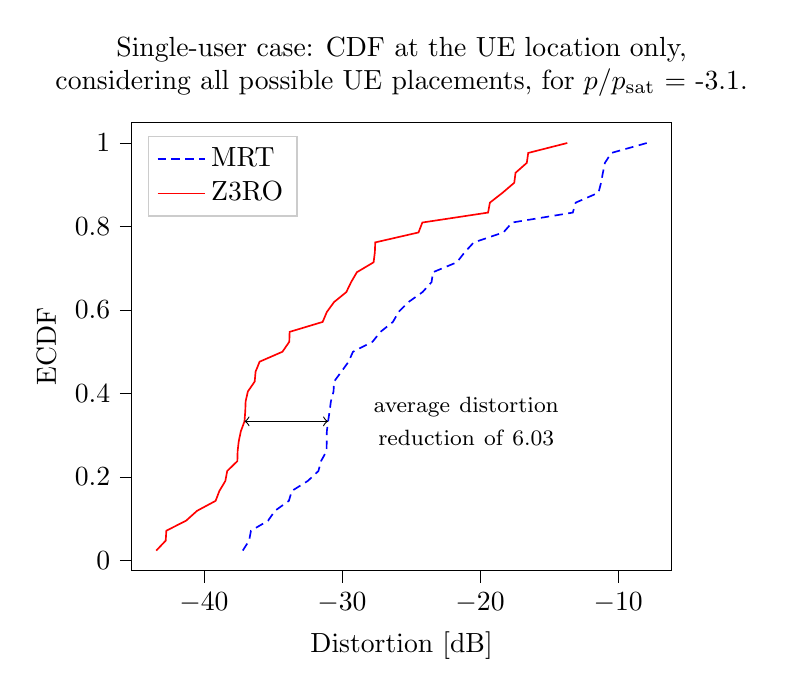
\begin{tikzpicture}
\usetikzlibrary{arrows}
\begin{axis}[
legend cell align={left},
legend style={
  fill opacity=0.8,
  draw opacity=1,
  text opacity=1,
  at={(0.03,0.97)},
  anchor=north west,
  draw=white!80!black
},
tick align=outside,
tick pos=left,
align=center,
title={Single-user case: CDF at the UE location only,\\ considering all possible UE placements, for $p/p_{\mathrm{sat}}$ = \SI{-3.1}{\decibel}.},
x grid style={white!69.0196078431373!black},
xlabel={Distortion [dB]},
xmin=-45.2243126655, xmax=-6.1413110045,
xtick style={color=black},
y grid style={white!69.0196078431373!black},
ylabel={ECDF},
ymin=-0.025, ymax=1.04880952380952,
ytick style={color=black}
]
\addplot [semithick, blue, densely dashed]
table {%
-inf 0
-37.18553658 0.0238095238095238
-36.72572707 0.0476190476190476
-36.58994019 0.0714285714285714
-35.35608716 0.0952380952380952
-34.85414298 0.119047619047619
-33.84721996 0.142857142857143
-33.6309251 0.166666666666667
-32.47749591 0.19047619047619
-31.70596021 0.214285714285714
-31.5170975 0.238095238095238
-31.11774034 0.261904761904762
-31.10409607 0.285714285714286
-31.09613145 0.30952380952381
-31.00703795 0.333333333333333
-30.89565503 0.357142857142857
-30.80366383 0.380952380952381
-30.61134488 0.404761904761905
-30.57221941 0.428571428571429
-30.04255593 0.452380952380952
-29.51967979 0.476190476190476
-29.2046821 0.5
-27.79023783 0.523809523809524
-27.21364097 0.547619047619048
-26.31058241 0.571428571428571
-25.90072046 0.595238095238095
-25.18270421 0.619047619047619
-24.16712635 0.642857142857143
-23.51445364 0.666666666666667
-23.4101193 0.69047619047619
-21.67819516 0.714285714285714
-21.11736534 0.738095238095238
-20.45465858 0.761904761904762
-18.30880988 0.785714285714286
-17.67791422 0.80952380952381
-13.28218097 0.833333333333333
-13.07683035 0.857142857142857
-11.42175702 0.880952380952381
-11.23769557 0.904761904761905
-11.10477553 0.928571428571428
-10.95691864 0.952380952380952
-10.49235577 0.976190476190476
-7.91781108 1
};
\addlegendentry{MRT}
\addplot [semithick, red]
table {%
-inf 0
-43.44781259 0.0238095238095238
-42.76557265 0.0476190476190476
-42.7194993 0.0714285714285714
-41.29485982 0.0952380952380952
-40.49281979 0.119047619047619
-39.15193236 0.142857142857143
-38.87689665 0.166666666666667
-38.4472139 0.19047619047619
-38.31140038 0.214285714285714
-37.5758416 0.238095238095238
-37.55681245 0.261904761904762
-37.47559473 0.285714285714286
-37.32388878 0.30952380952381
-37.06042408 0.333333333333333
-37.00381851 0.357142857142857
-36.97777459 0.380952380952381
-36.81685422 0.404761904761905
-36.32016075 0.428571428571429
-36.25664365 0.452380952380952
-35.9643312 0.476190476190476
-34.31145667 0.5
-33.81534644 0.523809523809524
-33.79121539 0.547619047619048
-31.39942037 0.571428571428571
-31.09611943 0.595238095238095
-30.5721725 0.619047619047619
-29.68600162 0.642857142857143
-29.33972238 0.666666666666667
-28.92015337 0.69047619047619
-27.70878267 0.714285714285714
-27.61913442 0.738095238095238
-27.5902538 0.761904761904762
-24.45914377 0.785714285714286
-24.17786613 0.80952380952381
-19.41816287 0.833333333333333
-19.28758523 0.857142857142857
-18.36458937 0.880952380952381
-17.52243157 0.904761904761905
-17.43133827 0.928571428571428
-16.61575436 0.952380952380952
-16.51219026 0.976190476190476
-13.68145225 1
};
\draw[<->] (-37.06042408,0.333333333333333) -- (-31.00703795,0.333333333333333);
\node[text width=3cm] at (-21.0,0.33333333333) {\footnotesize average distortion reduction of \SI{6.03}{\decibel}};
\addlegendentry{Z3RO}
\end{axis}


\end{tikzpicture}
